\documentclass{article}
\usepackage[utf8]{inputenc}
\usepackage{graphicx}
\usepackage{amsmath }
\usepackage{amssymb}
\usepackage{subcaption}
\usepackage{float}
\usepackage{mathtools}
\usepackage{algorithm}
\usepackage{algorithmic}
\usepackage{multirow}
\setcounter{section}{0}


\usepackage{cleveref} %referencing figures, equations and tables
\crefformat{figure}{Figure.~#2#1#3}
\crefformat{equation}{Eq.~#2#1#3}
\crefformat{table}{Table.~#2#1#3}
\crefformat{appendix}{Appendix.~#2#1#3}
\crefformat{section}{Section.~#2#1#3}

\title{TaperedBeam Static Analysis}
\author{Amir Baharvand }
\date{}

\begin{document}

\maketitle

\section{Problem Statement}
A cantilever tapered beam is shown in \cref{fig:beam}. As is seen, the beam undergoes a uniaxial compressive pressure at its right-end and its radius decreases linearly from 20mm to 10mm along the $x$-axis. The material behavior is elasto-plastic and is given in \cref{eq:elasto_plastic} and illustrated in \cref{fig:stress_strain}.

\begin{equation}
    \sigma(\epsilon) = 
    \begin{cases}
    E \epsilon & \sigma(\epsilon) \le \sigma_y\\ 
    \sigma_y \left( \dfrac{E \epsilon}{\sigma_y} \right)^{0.4} & \sigma(\epsilon) > \sigma_y
    \end{cases}
    \label{eq:elasto_plastic}
\end{equation}

where $\sigma$ and $\epsilon$ denote stress and strain, respectively. $E$ is Young's modulus and $\sigma_y$ is the yielding stress. The corresponding values are $E$=210GPa and $\sigma$=200MPa. The applied load magnitude is 1.5$\sigma_y$\\

\cref{fig:beam_fem} represents the numerical model of the tapered beam. The numerical model is built upon the following hypothesis.

\begin{enumerate}
    \item The beam undergoes uniaxial loading; hence, the beam element is reduced to a bar element.
    \item The tapered beam is reduced to a beam with a constant cross-section over the $x$-axis. A schematic representation is given with dashed lines in \cref{fig:beam_fem}.
    \item Boundary conditions are further simplified by removing the displacement in the $y$-direction.
    \item The applied stress is replaced by its equivalent point load.
    \item The effect of body force and traction are neglected and the numerical model only supports point loads.
\end{enumerate}

As a result, the tapered beam reduces to a beam with a constant cross-section that can be solved numerically using a bar element.

\begin{figure}[H]
    \centering
        \begin{subfigure}{0.49\textwidth}
            \includegraphics[width=1\linewidth]{figures/beam.pdf} 
            \caption{The cantilever tapered beam.}
            \label{fig:beam}
        \end{subfigure}
        \begin{subfigure}{0.49\textwidth}
            \includegraphics[width=1\linewidth]{figures/beam_fem.eps} 
            \caption{The Numerical model with constant radius of 30 mm.}
            \label{fig:beam_fem}
        \end{subfigure}
    \caption{The geometry, coordinate system  and boundary condition of the cantilever tapered beam under uniaxial loading.}
    \label{fig:beam_problem}
\end{figure}

\begin{figure}[H]
    \centering
    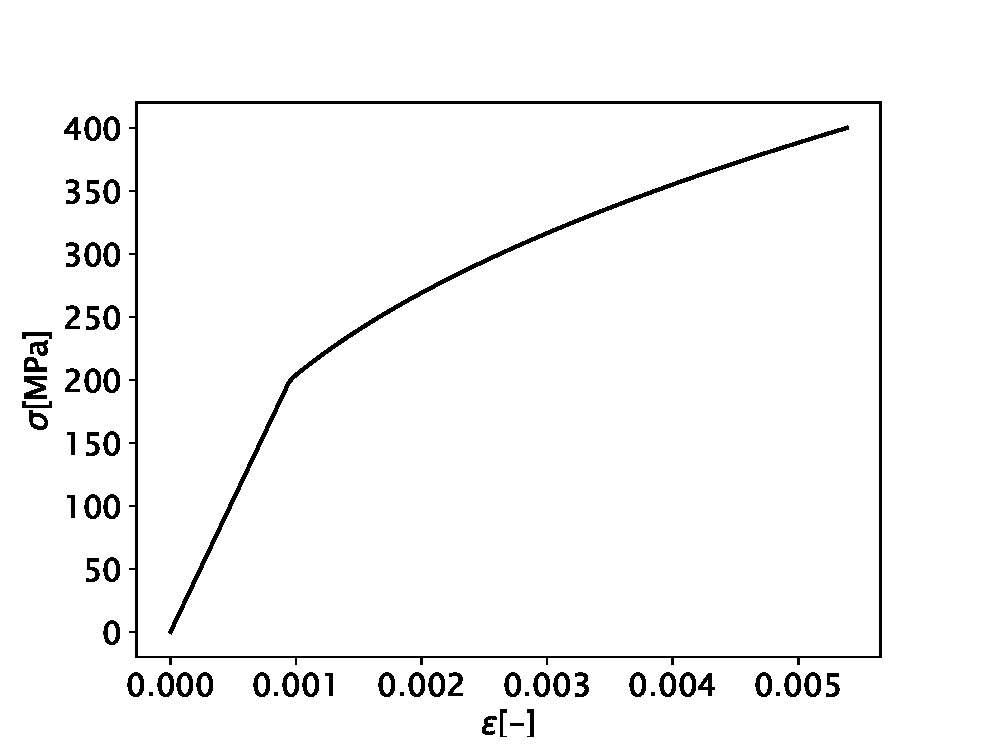
\includegraphics[width = 0.6\textwidth ]{figures/stress_strain.eps}
    \caption{The stress-strain curve from \cref{eq:elasto_plastic}.}
    \label{fig:stress_strain}
\end{figure}

\section{Finite Element Method}
The numerical model utilized in the present problem is Finite Element Method(FEM) and is developed base on the based on the virtual work principle. Finally, the results from the self-developed code, \texttt{mnb1c.py}\footnote{Material Nonlinearity Beam element one-dimensional Code} are compared with the commercial FEM code, Abaqus at the end of this report. 

\subsection{\texttt{mnb1c.py} Solver}
To satisfy the equilibrium \texttt{mnb1c.py} is combined with an iterative algorithm known as Implicit method. Here, the Newton-Raphson (NR) the Modified Newton-Raphson (MNR) are invoked. Such methods are invoked when one needs to derive the displacement from the applied load. Such methods do not depend on the increment size; however, implicit methods are computationally expensive due to the stiffness matrix factorization which is enhanced in the MNR.

\subsubsection{Newton-Raphson Method}
The pseudocode of the NR method is provided in \cref{alg:nr} and depicted in \cref{fig:nr_procedure} for two load increments. $\boldsymbol{K}$ is stiffness matrix, $\boldsymbol{R_{int}}$ is internal force vector, $\boldsymbol{R}$ is residual force vector, $\boldsymbol{D}$ is global displacement vector, $\boldsymbol{dD}$ is displacement vector for each load increment, $\boldsymbol{P}$ is global load vector and $\boldsymbol{\Delta P}$ is load vector for each load increment. The stiffness matrix factorization is performed in each iteration within an individual increment. To solve for displacement, different methods, for instance the LU factorization (as used in the present report) can be utilized.

\begin{algorithm}[ht]
\caption{Newton-Raphson pseudocode (B.C: Boundary Condition).}
\begin{algorithmic} 
\ENSURE $e = 1E-11$, $\boldsymbol{R} = 0$, $\boldsymbol{dD} = 0$,  $\boldsymbol{D} = 0$
\FOR{Load increment ($n$)}
    \FOR{Iteration}
        \STATE $\boldsymbol{K}$ = 0
        \STATE $\boldsymbol{R_{int}}$ = 0
        \STATE Compute $\boldsymbol{R_{int}}$
        \STATE Compute $R = \boldsymbol{R_{int} - n \Delta P}$
        \STATE Apply B.C on $\boldsymbol{R}$
        \IF{norm($\boldsymbol{R}$) $\le$ $\epsilon$ norm($P$)}
            \STATE break
        \ENDIF
        \STATE Compute $\boldsymbol{K}$
        \STATE Apply B.C on $\boldsymbol{K}$
        \STATE Solve $\boldsymbol{dD} = \boldsymbol{K}^{-1} \boldsymbol{R}$
        \STATE Factorize $\boldsymbol{K}$
        \STATE $\boldsymbol{D} = D + dD$
    \ENDFOR
    \STATE Write $\boldsymbol{D}$
    \STATE Write $n \Delta P$
\ENDFOR
\end{algorithmic}
\label{alg:nr}
\end{algorithm}

\begin{figure}[ht]
    \centering
        \begin{subfigure}{0.64\textwidth}
            \includegraphics[width=1\linewidth]{figures/nr1.pdf} 
            \caption{The first load increment with three iterations}
            \label{fig:nr1}
        \end{subfigure}
        
        \begin{subfigure}{0.64\textwidth}
            \includegraphics[width=1\linewidth]{figures/nr2.pdf} 
            \caption{The second load increment with two iterations}
            \label{fig:nr2}
        \end{subfigure}
        
        \begin{subfigure}{0.64\textwidth}
            \includegraphics[width=1\linewidth]{figures/nr3.pdf} 
            \caption{The first two load increments with their corresponding displacements.}
            \label{fig:nr3}
        \end{subfigure}
    \caption{An schematic representation of the Newton-Raphson method for two load increments. $K$ is the stiffness matrix, $R$ is the residual vector from equilibrium, $P$ is the load and $u$ is the displacement. The subscripts $a$ and $b$ denote the trial displacement while the numbered subscripts denote the final displacement for the corresponding load increment.}
    \label{fig:nr_procedure}
\end{figure}

\subsubsection{Modified Newton-Raphson Method}
In this method, the expensive process of stiffness matrix factorization is boosted by removing this step from each iteration. The MNR method performs the stiffness matrix factorization outside the iteration loop and use it later for solving the displacement. As a result, MNR requires more iteration in comparison to the NR. The MNR pseudocode is given in \cref{alg:mnr} and illustrated in \cref{fig:mnr_procedure} for two load increments.

\begin{algorithm}[ht]
\caption{Modified Newton-Raphson pseudocode.}
\begin{algorithmic} 
\ENSURE $e = 1E-11$, $\boldsymbol{R} = 0$, $\boldsymbol{dD} = 0$,  $\boldsymbol{D} = 0$
\FOR{Load increment ($n$)}
    \STATE Compute $\boldsymbol{K_{inc}}$
    \STATE Factorize $\boldsymbol{K_{inc}}$
    \STATE Apply B.C on $\boldsymbol{K_{inc}}$
    \FOR{Iteration}
        \STATE $\boldsymbol{K}$ = 0
        \STATE $\boldsymbol{R_{int}}$ = 0
        \STATE Compute $\boldsymbol{R_{int}}$
        \STATE Compute $R = \boldsymbol{R_{int} - n \Delta P}$
        \STATE Apply B.C on $\boldsymbol{R}$
        \IF{norm($\boldsymbol{R}$) $\le$ $\epsilon$ norm($P$)}
            \STATE break
        \ENDIF
        \STATE Solve $\boldsymbol{dD} = \boldsymbol{K_{inc}}^{-1} \boldsymbol{R}$
        \STATE $\boldsymbol{D} = D + dD$
    \ENDFOR
    \STATE Write $\boldsymbol{D}$
    \STATE Write $n \Delta P$
\ENDFOR
\end{algorithmic}
\label{alg:mnr}
\end{algorithm}

\begin{figure}[ht]
    \centering
        \begin{subfigure}{0.64\textwidth}
            \includegraphics[width=1\linewidth]{figures/mnr1.pdf} 
            \caption{The first load increment with five iterations}
            \label{fig:mnr1}
        \end{subfigure}
        
        \begin{subfigure}{0.64\textwidth}
            \includegraphics[width=1\linewidth]{figures/mnr2.pdf} 
            \caption{The second load increment with four iterations}
            \label{fig:mnr2}
        \end{subfigure}
        
        \begin{subfigure}{0.64\textwidth}
            \includegraphics[width=1\linewidth]{figures/mnr3.pdf} 
            \caption{The first two load increments with their corresponding displacements.}
            \label{fig:mnr3}
        \end{subfigure}
    \caption{An schematic representation of the Modified Newton-Raphson method for two load increments. $K$ is the stiffness matrix, $R$ is the residual vector from equilibrium, $P$ is the load and $u$ is the displacement. The Roman subscripts in $K$ denote the initial tangential stiffness matrix for each load increment. The numbered subscripts denote the final displacement for the corresponding load increment.}
    \label{fig:mnr_procedure}
\end{figure}

\subsubsection{Newton-Raphson vs. Modified Newton-Raphson}
\cref{tab:nr_vs_mnr} compares the number of iterations required for each load increment from the three NR, MNR and Abaqus NR for the beam problem in \cref{fig:beam_fem}. As expected, the MNR needs more iteration for each load increment compared to the NR method. The maximum number of iteration for the MNR occurs at the load increment 7 where the problem migrates from the elastic regime to the plastic and thus the codes requires more iterations to fulfill the equilibrium.\\

\begin{table}[H]
\caption{Non-tapered beam: Comparison between the number of iterations required for a 10-load increment (Fixed load increment activated in Abaqus).}
    \label{tab:nr_vs_mnr}
    \centering
    \begin{tabular}{cccc}
\hline
\multirow{2}{*}{\begin{tabular}[c]{@{}c@{}}Increment \\ Number\end{tabular}} & \multicolumn{3}{c}{Number of iterations}                                            \\ \cline{2-4} 
                                                                                 & Newton-Raphson & \begin{tabular}[c]{@{}c@{}}Modified \\  Newton-Raphson\end{tabular} & \begin{tabular}[c]{@{}c@{}}Abaqus \\  (Newton-Raphson)\end{tabular}\\ \hline
        1 & 1 & 1 & 1\\
        2 & 1 & 1 & 1\\
        3 & 1 & 1 & 1\\
        4 & 1 & 1 & 1\\
        5 & 1 & 1 & 1\\
        6 & 1 & 1 & 1\\
        7 & 4 & 52 & 2\\
        8 & 4 & 15 & 1\\
        9 & 4 & 14 & 2\\
        10 & 4 & 13 & 1\\ \hline
    \end{tabular}
\end{table}


\cref{tab:nr_vs_mnr_benchmark} compares the elapsed time for both the NR and MNR methods. The advantage of stiffness matrix factorization outside the iteration loop makes the MNR a suitable method for numerical problems with higher number of load increments. 

\begin{table}[H]
\caption{Non-tapered beam: Newton-Raphson vs. Modified Newton-Raphson benchmark}
\label{tab:nr_vs_mnr_benchmark}
\centering
\begin{tabular}{ccc}
\hline
\multirow{2}{*}{\begin{tabular}[c]{@{}c@{}}Number of \\ increments\end{tabular}} & \multicolumn{2}{c}{Elapsed time{[}s{]}}                                            \\ \cline{2-3} 
                                                                                 & Newton-Raphson & \begin{tabular}[c]{@{}c@{}}Modified \\  Newton-Raphson\end{tabular} \\ \hline
10                                                                               & 0.024          & 0.050                                        \\
100                                                                              & 0.161          & 0.175                                                              \\
1000                                                                             & 1.33           & 1.32                                                               \\
10000                                                                            & 12.7           & 11.9                                                               \\ 
100000                                                                            & 126           & 105                                                               \\ \hline
\end{tabular}
\end{table}


\subsection{Abaqus}
In this section, necessary steps for the numerical modeling in Abaqus are mentioned.

\subsubsection{Mechanical Properties}
The numerical model unit is set to SI unit in meters. \cref{tab:mat_prop} summarizes the mechanical properties of the beam.

\begin{table}[H]
    \centering
    \caption{Mechanical properties of the beam.}
    \begin{tabular}{l c c c} \hline
        Property & Symbol & Unit & Value \\ \hline
        Young's modulus & $E$& Pa & 2.1E11 \\
        Poisson's ratio & $\nu$ & - & 0.3 \\
        Yielding stress & $\sigma_y$ & Pa & 2E08 \\ \hline
    \end{tabular} 
    \label{tab:mat_prop}
\end{table}

The plastic behavior is imported as a table in Abaqus. A Python script is developed which can generate a table of plastic properties which can be imported into Abaqus. \cref{tab:plastic_prop} summarizes the input file for the plastic behavior in Abaqus.

\begin{table}[H]
    \centering
    \caption{Plastic behavior of the beam defined in Abaqus.}
    \label{tab:plastic_prop}
    \begin{tabular}{ll} \hline
        Yield stress[Pa] & Plastic strain[-] \\ \hline
        2E08 & 0 \\
        2.5E08 & 0.0007114 \\
        3E08 & 0.0016721 \\
        3.5E08 & 0.0029060 \\
        4E08 & 0.0044351  \\ \hline
    \end{tabular}
\end{table}

\subsubsection{Solver}
The solver for this problem is set to \textbf{Static, General} because the problem is linear static (no contact, boundary conditions do not change with time). As mentioned, the solver invokes the Newton-Raphson method.

\subsubsection{Element Type}
The B21 element (a 2-node linear beam with one integration point in middle in two-dimension) and B31 element (a 2-node linear beam with one integration point in middle in three-dimension) with shear-flexible (based on Timoshenko beam theory) formulation are selected for the Abaqus numerical modeling in the two and three-dimension, respectively. The B21, B31 and the bar element from \texttt{mnb1c.py} are illustrated for convenience in \cref{fig:element}

\begin{figure}[H]
    \centering
    \includegraphics[width = 1\textwidth ]{figures/all_elements.pdf}
    \caption{(a) The bar element used in \texttt{mnb1c.py}. (b) The B21 element. (c) The B31 element. $u$, $v$ and $w$ are the nodal displacement in the $x$, $y$ and $z$-direction and $\theta$ is the rotation. Subscripts 1 and 2 denote the node number.}
    \label{fig:element}
\end{figure}

\subsection{Result and Discussion}
\subsubsection{Non-tapered Beam}
\cref{fig:result_non_tapered_beam} shows the load-displacement plot for the right end of the beam (node 5 in \cref{fig:beam_fem}). For the FEM analysis using Abaqus, two numerical models are developed. One uses 5 points for the definition of plastic behavior (see \cref{tab:plastic_prop}) while another uses 50 points. The results from both the NR and MNR coincide with the analytical model as both the NR and MNR utilizes \cref{eq:elasto_plastic} for the relation between the stress and strain and \cref{eq:tangential_stiffness} tangential stiffness in the plastic region. 

\begin{equation}
    \dfrac{\text{d}\sigma(\epsilon)}{\text{d}\epsilon} = 
    \begin{cases}
     E & \sigma \le \sigma_y\\ 
    \dfrac{0.4 E}{\left( \dfrac{E \epsilon}{\sigma_y} \right)^{0.6}} & \sigma > \sigma_y
    \end{cases}
    \label{eq:tangential_stiffness}
\end{equation}

Abaqus follows the analytical solution in the elastic regime; nevertheless, it overestimates the displacement for a certain load increment. Increasing the number of plastic behavior point to 50 enables Abaqus to perform a better interpolation between the given points in the transition zone (from elastic to plastic). Abaqus is incapable of solving the problem with 10 load increments and crashes for fixed load increment. Thus, the increment size is set to "Automatic". It appears that higher number of points for the plastic regime only improves the result in the elasto-plastic transition zone and does not affect the solution.

\begin{figure}[H]
    \centering
    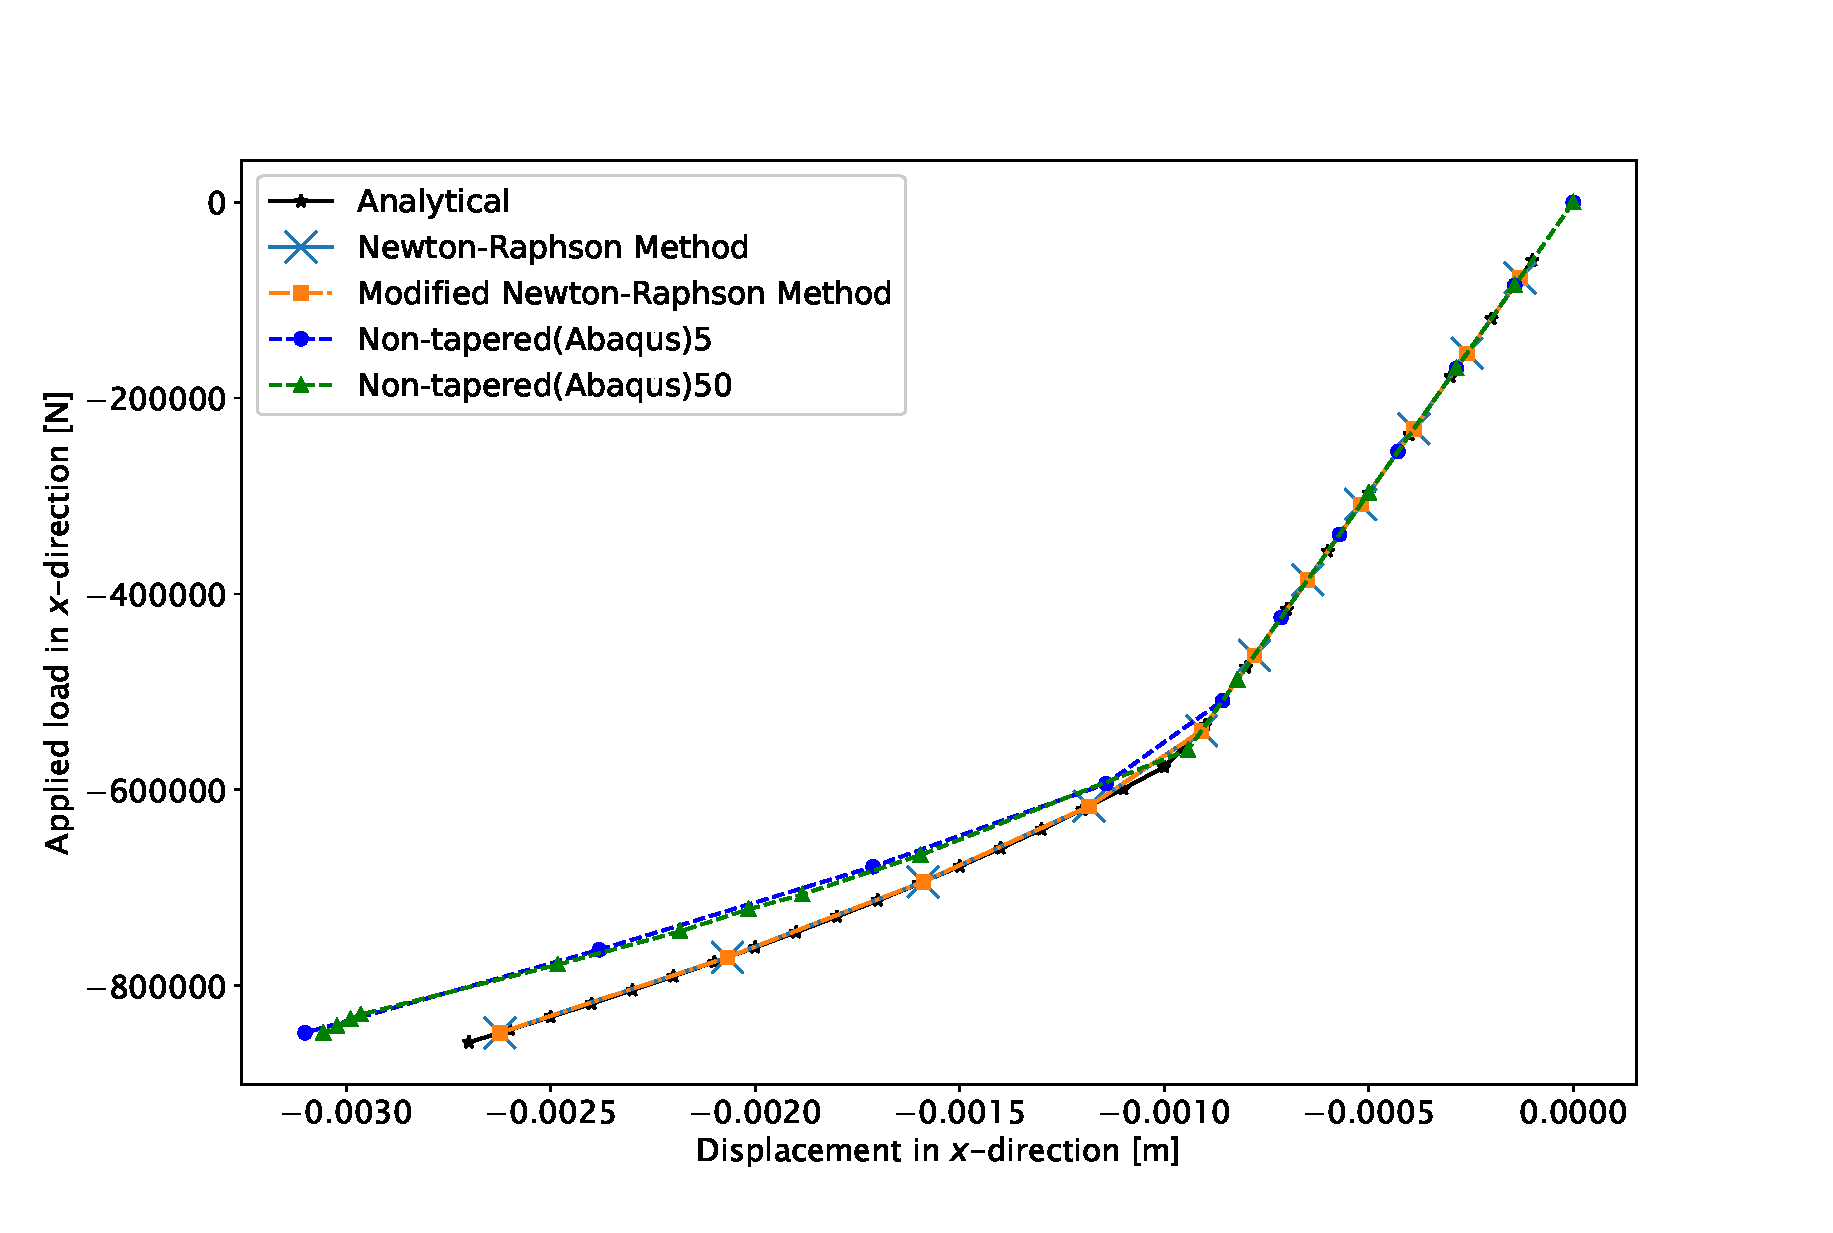
\includegraphics[width = 1\textwidth ]{figures/comparison_non_tapered.eps}
    \caption{Non-tapered beam: Load vs. displacement (along $x$-axis) plot of right-end of the beam (node 5 in \cref{fig:beam_fem}).}
    \label{fig:result_non_tapered_beam}
\end{figure}

\subsubsection{Tapered Beam}
The load-displacement plot for the tapered beam (see \cref{fig:tapered_beam}) is shown in \cref{fig:result_tapered_beam}.  \texttt{mnb1c.py} requires more load increment than the non-tapered version and the NR method crashes for load increments less than 10. \cref{tab:nr_vs_mnr_tapered} list the iterations for each load increments in \texttt{mnb1c.py}.

\begin{figure}[H]
    \centering
    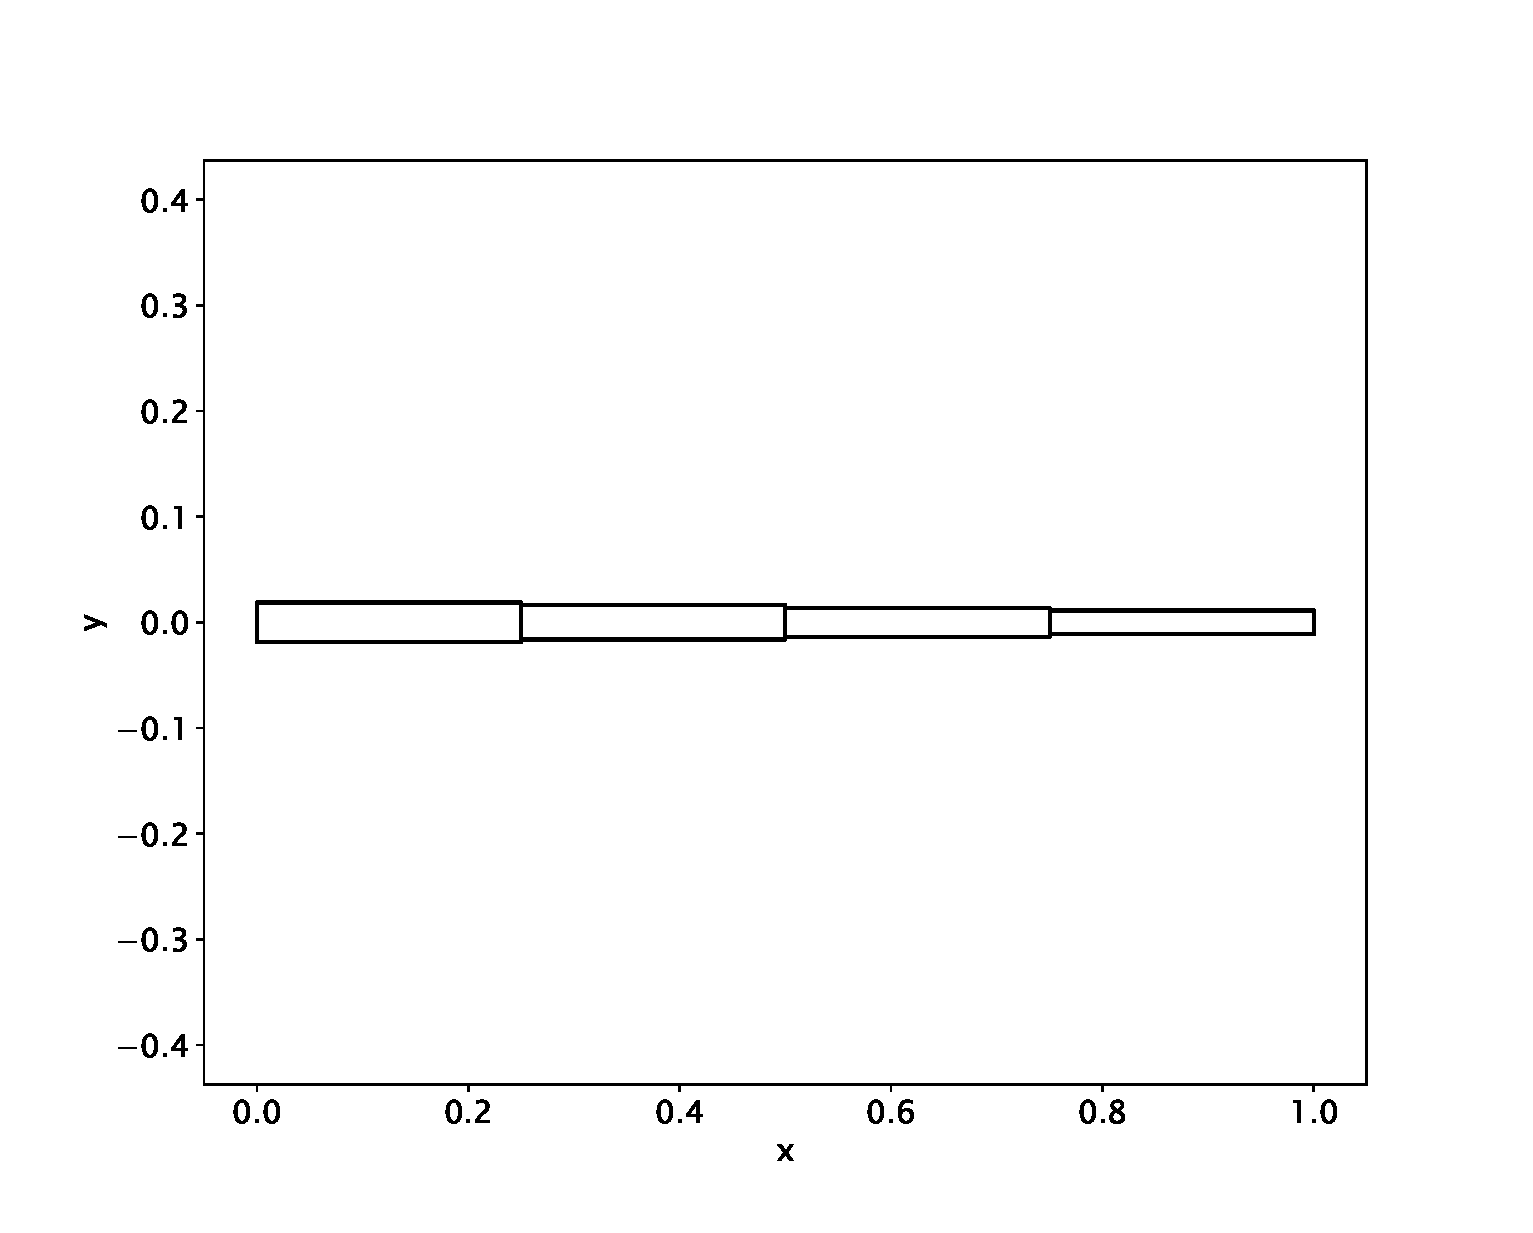
\includegraphics[width = 0.6\textwidth ]{figures/tapered_beam.eps}
    \caption{The simplified version of the tapered beam from \cref{fig:beam} (Axes units depends on the initial parameter definition. Here both axes units are meters.)}
    \label{fig:tapered_beam}
\end{figure}

\begin{table}[H]
\caption{Tapered beam: Comparison between the number of iterations required for an 11-load increment in \texttt{mnb1c.py}.}
    \label{tab:nr_vs_mnr_tapered}
    \centering
    \begin{tabular}{ccc}
\hline
\multirow{2}{*}{\begin{tabular}[c]{@{}c@{}}Increment \\ Number\end{tabular}} & \multicolumn{2}{c}{Number of iterations}                                            \\ \cline{2-3} 
                                                                                 & Newton-Raphson & \begin{tabular}[c]{@{}c@{}}Modified \\  Newton-Raphson\end{tabular} \\ \hline
        1 & 1 & 1 \\
        2 & 1 & 1 \\
        3 & 8 & 224 \\
        4 & 10 & 110 \\
        5 & 10 & 42 \\
        6 & 13 & 72 \\
        7 & 10 & 35 \\
        8 & 9 & 93 \\
        9 & 4 & 14 \\
        10 & 4 & 13 \\
        11 & 4 & 13 \\ \hline
    \end{tabular}
\end{table}

Unlike Abaqus, \texttt{mnb1c.py} is able to solve the problem (see \cref{fig:result_tapered_beam}) to the last load increment which may be attributed to the analytical equations for and the stress-strain (\cref{eq:elasto_plastic}) tangential stiffness matrix (\cref{eq:tangential_stiffness}). Abaqus solver crashes right before the transition zone and increasing the number of plastic behavior to 50 results in crashing the solution procedure.

\begin{figure}[H]
    \centering
    \includegraphics[width = 1\textwidth ]{figures/comparison_tapered.eps}
    \caption{Tapered beam: Load vs. displacement (along $x$-axis) plot of right-end of the beam (node 5 in \cref{fig:beam_fem}). Abaqus results are provided up to the last solve increment.}
    \label{fig:result_tapered_beam}
\end{figure}


%\newpage
%\bibliography{ref}
%\bibliographystyle{ieeetr}

\end{document}